%%%%%%%%%%%%%%%%%%%%%%%%%%%%%%%%%%%%%%%%%%%%%%%%%%%%%%%%%%%%%%%%%%%%%%%%%%%%%%%%
% UVic Thesis/Dissertation/Report LaTeX Document Class Template
% Created by Michael D. Adams (mdadams@ece.uvic.ca)
%%%%%%%%%%%%%%%%%%%%%%%%%%%%%%%%%%%%%%%%%%%%%%%%%%%%%%%%%%%%%%%%%%%%%%%%%%%%%%%%

% UVic Thesis Document Class Options
% ==================================
%
% In addition to the options provided by the book document class, the
% uvicthesis document class also supports the following options:
%
% review
%     Enable review mode (e.g., use double spacing).
%     This generally looks ugly but is very helpful if a reviewer
%     (e.g., supervisor) wants to write annotations on the pages
%     of the document in order to indicate corrections/revisions that
%     should be made.

% IMPORTANT NOTES:
%
% The University of Victoria changed the rules for theses at some point in
% time to require pagination for one-sided printing.  As a result, the
% oneside option must be used.
%
% The University of Victoria should allow (unless the rules have changed
% since the time of this writing) font sizes of 10, 11, or 12 point.
% There are numerous tradeoffs in the choice of font size:
%   - larger fonts often make typesetting more difficult because
%     many tables/figures/equations/listings fall outside the margins of
%     the page
%   - larger fonts are easier for people with poor eyesight to read
%     when viewing a document on a small display
% So, generally, larger fonts have both advantages and disadvantages.
% Personally, I would recommend using a larger font as long as you
% do not encounter problems with tables/equations/figures not fitting
% on the page.

\documentclass[
  %10pt,
  11pt, % NOTE: Perhaps, this is the best compromise for font size?
  %12pt,
  oneside,
  %review, % Uncomment for review mode.  (See above for details.)
]{uvicthesis}

%%%%%%%%%%%%%%%%%%%%%%%%%%%%%%%%%%%%%%%%%%%%%%%%%%%%%%%%%%%%%%%%%%%%%%%%%%%%%%%%
% Information about the author and document.
%%%%%%%%%%%%%%%%%%%%%%%%%%%%%%%%%%%%%%%%%%%%%%%%%%%%%%%%%%%%%%%%%%%%%%%%%%%%%%%%

% The title of the document.
\title{The Answer to the Ultimate Question About the Life, the Universe, and
  Everything}

% The author of the document.
\author{Arthur Dent}

% The department of the author.
\department{Department of Electrical and Computer Engineering}

% The degrees already held by the author.
\degrees{%
B.A.Sc., Massachusetts Institute of Technology, 2000 \\
M.A.Sc., University of Waterloo, 2004
}

% The year of publication of the document.
\year{2019}

% The document type (i.e., thesis, dissertation, or report).
%\doctype{Report}
%\doctype{Thesis}
\doctype{Dissertation}

% The type of degree associated with this document.
%\degreetype{Master of Engineering}
%\degreetype{Master of Applied Science}
\degreetype{Doctor of Philosophy}

% The members of the Supervisory Committee.
\newcommand{\committee}{
  \panellist{Dr.\ Jane Doe}{Supervisor}
    {Department of Electrical and Computer Engineering}
  \panellist{Dr.\ John Doe}{Departmental Member}
    {Department of Electrical and Computer Engineering}
  \panellist{Dr.\ Anon Y.\ Mous}{Outside Member}
    {Department of Computer Science}
}

%%%%%%%%%%%%%%%%%%%%%%%%%%%%%%%%%%%%%%%%%%%%%%%%%%%%%%%%%%%%%%%%%%%%%%%%%%%%%%%%
% Some miscellaneous initialization.
%%%%%%%%%%%%%%%%%%%%%%%%%%%%%%%%%%%%%%%%%%%%%%%%%%%%%%%%%%%%%%%%%%%%%%%%%%%%%%%%

\usetikzlibrary{
  arrows.meta,
  backgrounds,
  graphs,
  positioning,
  shadows,
  shapes,
  quotes,
  shapes.multipart,
}

%%%%%%%%%%%%%%%%%%%%%%%%%%%%%%%%%%%%%%%%%%%%%%%%%%%%%%%%%%%%%%%%%%%%%%%%%%%%%%%%
% Some setup for the listings package.
%%%%%%%%%%%%%%%%%%%%%%%%%%%%%%%%%%%%%%%%%%%%%%%%%%%%%%%%%%%%%%%%%%%%%%%%%%%%%%%%

% Flexible columns are used in an attempt to avoid extra spaces being
% inserted into listings.
\lstset{columns=flexible}

\lstdefinestyle{cxx}{
  language = C++,
  basicstyle = {\ttfamily},
  showspaces = false,
  showtabs = false,
  showstringspaces = false,
  escapechar = @,
  escapebegin = \rm,
  xleftmargin = 4ex,
  xrightmargin = 0ex,
  tabsize = 4,
}

\lstdefinestyle{numbers}
  {numbers=left,stepnumber=1,numberstyle=\tiny,numbersep=10pt}
\lstdefinestyle{nonumbers}{numbers=none}

%%%%%%%%%%%%%%%%%%%%%%%%%%%%%%%%%%%%%%%%%%%%%%%%%%%%%%%%%%%%%%%%%%%%%%%%%%%%%%%%
% Some other convenience macros.
%%%%%%%%%%%%%%%%%%%%%%%%%%%%%%%%%%%%%%%%%%%%%%%%%%%%%%%%%%%%%%%%%%%%%%%%%%%%%%%%

\newcommand{\term}[1]{\index{#1}{#1}}

%%%%%%%%%%%%%%%%%%%%%%%%%%%%%%%%%%%%%%%%%%%%%%%%%%%%%%%%%%%%%%%%%%%%%%%%%%%%%%%%
% End of the preamble.
%%%%%%%%%%%%%%%%%%%%%%%%%%%%%%%%%%%%%%%%%%%%%%%%%%%%%%%%%%%%%%%%%%%%%%%%%%%%%%%%

\begin{document}

%%%%%%%%%%%%%%%%%%%%%%%%%%%%%%%%%%%%%%%%%%%%%%%%%%%%%%%%%%%%%%%%%%%%%%%%%%%%%%%%
% Front matter (i.e., title page, abstract, table of contents, etc.)
%%%%%%%%%%%%%%%%%%%%%%%%%%%%%%%%%%%%%%%%%%%%%%%%%%%%%%%%%%%%%%%%%%%%%%%%%%%%%%%%

\frontmatter

\maketitle
\begin{abstract}
This is the abstract.
\end{abstract}

\tableofcontents
\listoftables
\listoffigures
\lstlistoflistings
\preface
\begin{acknowledgments}
I acknowledge no one.
\end{acknowledgments}

This book is dedicated to Douglas Adams.


%%%%%%%%%%%%%%%%%%%%%%%%%%%%%%%%%%%%%%%%%%%%%%%%%%%%%%%%%%%%%%%%%%%%%%%%%%%%%%%%
% Main matter (i.e., chapters and appendices).
%%%%%%%%%%%%%%%%%%%%%%%%%%%%%%%%%%%%%%%%%%%%%%%%%%%%%%%%%%%%%%%%%%%%%%%%%%%%%%%%

\mainmatter

\chapter{Introduction}

\section{Overview}

This is the introduction.
Some terms for the index are as follows:
\term{foo}, \term{bar}, \term{baz}.

\section{Lipsum}

\lipsum
\lipsum
\lipsum
\lipsum

\chapter{Background}

\section{The Hitchhiker's Guide to the Galaxy}

You are not intimately familiar with the
``The Hitchhiker's Guide to the Galaxy'' \cite{Adams_1980a}?
Surely, you jest.

\begin{figure}
\begin{minipage}{\textwidth}\centering%
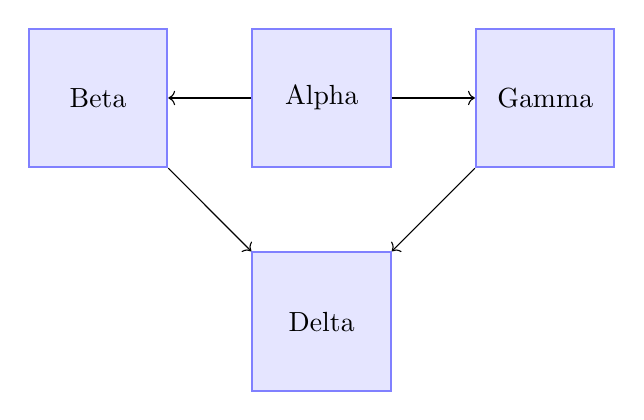
\begin{tikzpicture}%
\tikzstyle{thing}=[rectangle,draw=blue!50,fill=blue!10,thick,minimum size=5em]
\node[thing] (a) {Alpha};
\node[thing] (b) [left=3em of a] {Beta};
\node[thing] (c) [right=3em of a] {Gamma};
\node[thing] (d) [below=3em of a] {Delta};
\draw[->] (a) -- (b);
\draw[->] (a) -- (c);
\draw[->] (b) -- (d);
\draw[->] (c) -- (d);
\end{tikzpicture}%
\end{minipage}%
\caption{Gratuitous figure.}
\end{figure}

\section{Stuff}

\begin{lemma}[Title]
\lipsum[1]
\end{lemma}

\begin{proposition}[Title]
\lipsum[1]
\end{proposition}

\begin{corollary}[Title]
\lipsum[1]
\end{corollary}

\begin{definition}[Term]
\lipsum[1]
\end{definition}

\begin{theorem}[Title]
The most important number is 42.
\end{theorem}
\begin{proof}
The proof is obvious and is omitted here.
\end{proof}

\begin{example}[Title]
\lipsum[1]
\end{example}


\section{Lipsum}

\lipsum
\lipsum
\lipsum
\lipsum

\chapter{Proposed Method}

\section{Proposed Method}

I am not proposing anything.

\section{Lipsum}

\lipsum
\lipsum
\lipsum
\lipsum

\chapter{Results}

\section{Summary}

Results omitted due to lack of motivation.

\begin{figure}\centering%
\begin{minipage}{0.5\textwidth}\centering%
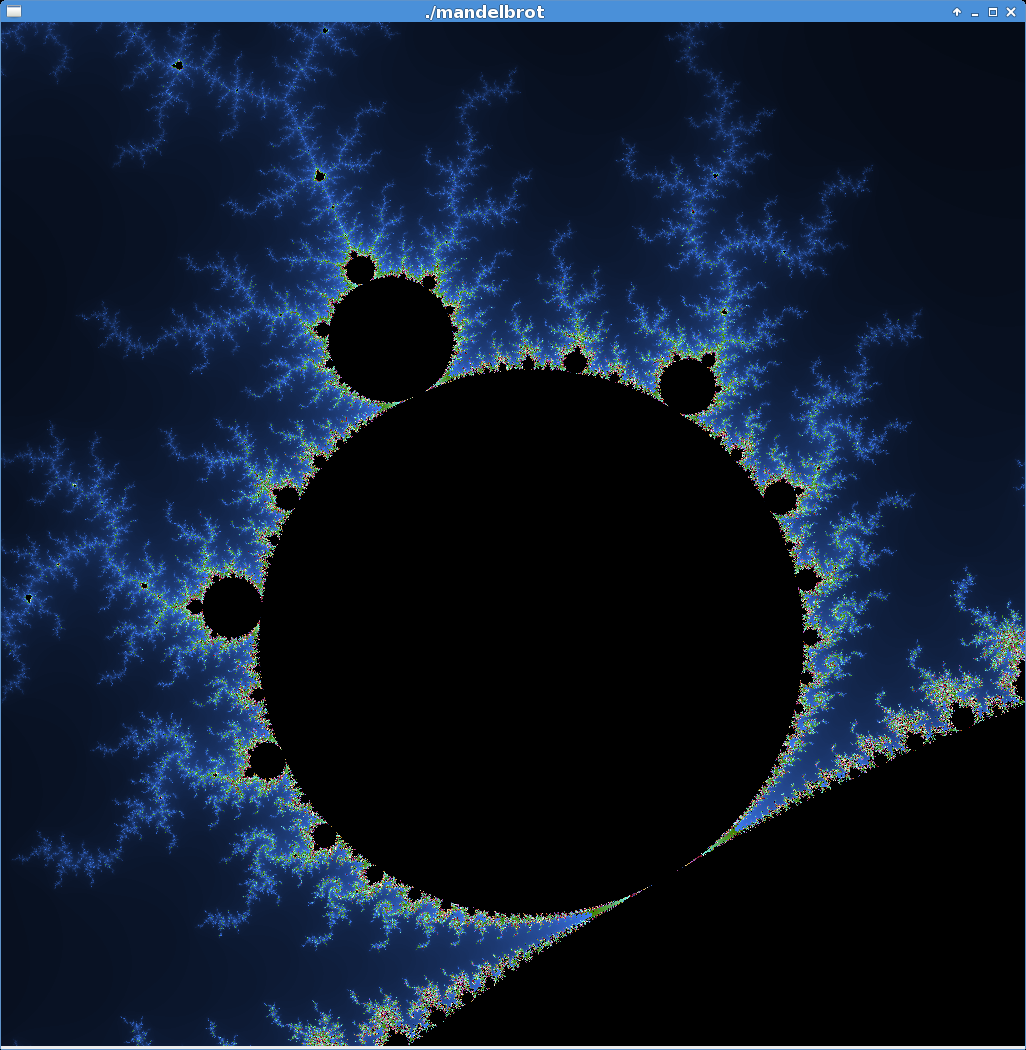
\includegraphics[width=0.98\textwidth]{figures/mandelbrot.png}
\\ (a)
\end{minipage}%
\begin{minipage}{0.5\textwidth}\centering%
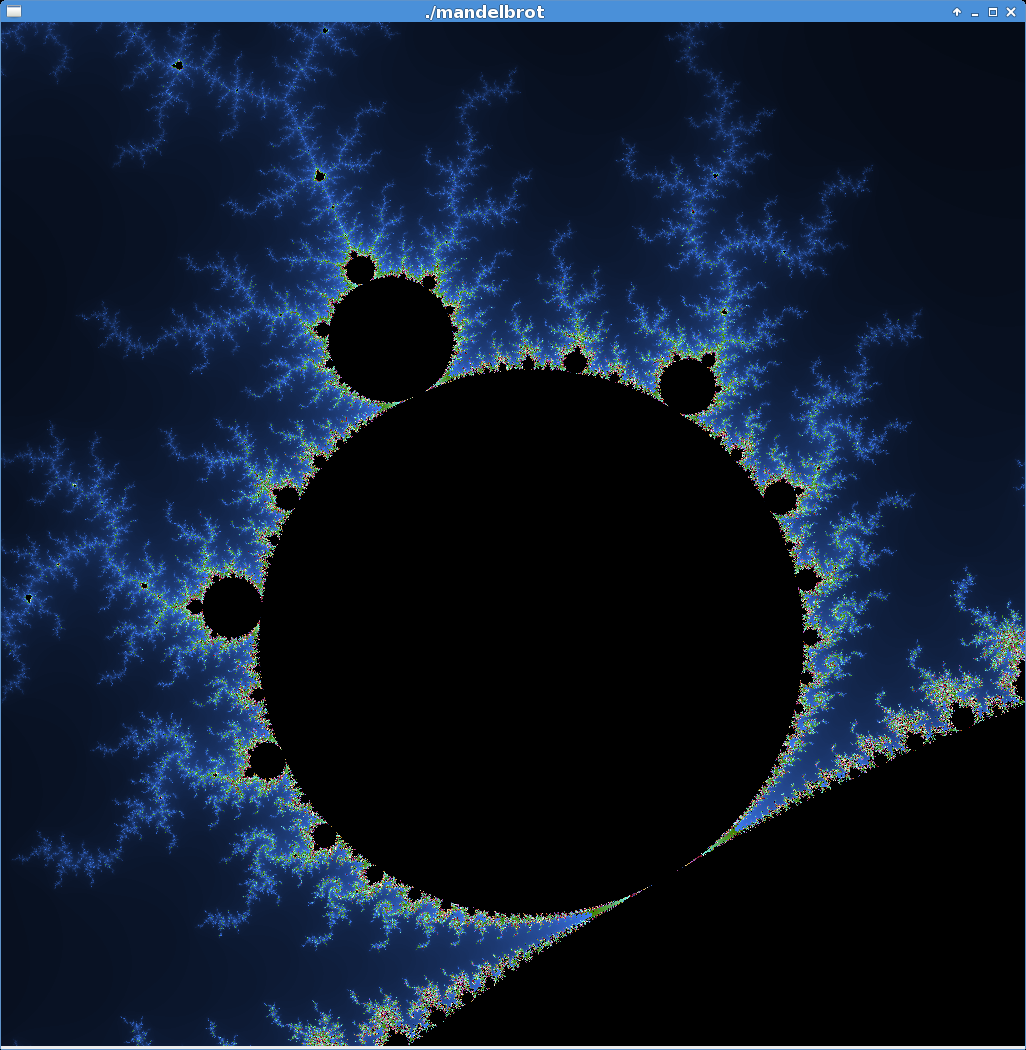
\includegraphics[width=0.98\textwidth]{figures/mandelbrot.png}
\\ (b)
\end{minipage}%
\caption{Gratuitous Mandebrot art.
(a)~Mandelbrot and (b)~Mandelbrot.}
\end{figure}

\begin{table}\centering%
\begin{tabular}{|l|l|}%
\hline
x & y \\
\hline
1 & 2 \\
3 & 4 \\
5 & 6 \\
\hline
\end{tabular}%
\caption{Another table}
\end{table}

\begin{lstlisting}[caption={Some caption.},frame=single]
This is a listing.
\end{lstlisting}

\lstinputlisting[caption={Some caption.},frame=single]{software/hello.cpp}

\section{Lipsum}

\lipsum
\lipsum
\lipsum
\lipsum

\chapter{Conclusions}

\section{Summary}

The answer is 42.

\section{Future Work}

What is the question to which 42 is the answer?

\section{Lipsum}

\lipsum
\lipsum
\lipsum
\lipsum


\appendix

\chapter{Some Appendix}

This is an appendix.


%%%%%%%%%%%%%%%%%%%%%%%%%%%%%%%%%%%%%%%%%%%%%%%%%%%%%%%%%%%%%%%%%%%%%%%%%%%%%%%%
% Back matter (i.e., bibliiography and index).
%%%%%%%%%%%%%%%%%%%%%%%%%%%%%%%%%%%%%%%%%%%%%%%%%%%%%%%%%%%%%%%%%%%%%%%%%%%%%%%%

\backmatter

\bibliographystyle{plain}
\bibliography{references}
\addcontentsline{toc}{chapter}{\indexname}
\printindex%
\cleardoublepage%

%%%%%%%%%%%%%%%%%%%%%%%%%%%%%%%%%%%%%%%%%%%%%%%%%%%%%%%%%%%%%%%%%%%%%%%%%%%%%%%%
% End of document.
%%%%%%%%%%%%%%%%%%%%%%%%%%%%%%%%%%%%%%%%%%%%%%%%%%%%%%%%%%%%%%%%%%%%%%%%%%%%%%%%

\end{document}
